\chapter{Results and Analysis}
\label{ch:ResultsAnalysis}
In this chapter, the performance of the trained models is analyzed and discussed. The main focus is on the final MLP regressor model, which was found to be the best performing model across multiple criteria. The selection of the MLP regressor is supported by the results shown in \autoref{fig:ModelSRCC}, which presents a parallel coordinate plot comparing the best-performing models across all seven criteria and the overall SRCC.\par
The parallel coordinate plot shows that the MLP regressor consistently performs better than the other models across all criteria. Although all models perform similarly for different criteria, no model stands out in a specific criterion. This could be because the same features were used for every criterion, with only the target labels differing. \par
\vspace{\baselineskip}
\noindent
In addition to the parallel coordinate plot, \autoref{table:srcc_results} summarizes the cross-dataset evaluation results, showing the generalizability of the models. The table lists the models in the left column and their evaluation results on the SCIN and Fitzpatrick (F17K) datasets in the right columns. This table shows how well the models, trained on one dataset, perform when evaluated on another, providing insights into their robustness and adaptability. All data were synthetically distorted through the pipeline to ensure consistent evaluation conditions. \par
\vspace{\baselineskip}
\noindent
Given these findings, the MLP regressor was chosen as the final model for further testing. The following sections will detail the performance of the MLP regressor on the test images, providing a clear analysis of its strengths and weaknesses in assessing image quality in teledermatology. \par

\section{Range of Distortion Values}
\label{sec:RangeDistortionValues}
The ranges of values for each distortion type were carefully chosen to reflect realistic scenarios for teledermatology  applications. Each distortion type was visualized individually to make sure they were appropriate. \autoref{sec:Degradation_Types} includes images that show each criterion with different distortion types and five severity levels. \par
\vspace{\baselineskip}
\noindent
It is important to note that images should not be normalized before viewing because normalization can make the images appear overly colorful and unrealistic. However, normalization is necessary during training and testing because the feature extraction backbone from ARNIQA\autocite{ARNIQA} was trained on ResNet50 with ImageNet images. This step helps the model accurately extract relevant features from the images. \par
\section{Model Performance}
\label{sec:ModelPerformance}
To fully understand the performance of the four different models with different architectures, a cross-dataset evaluation was done. \autoref{table:srcc_results} summarizes the overall Spearman’s Rank Correlation Coefficient (SRCC) on the synthetically distorted SCIN and Fitzpatrick datasets. This evaluation highlights how well the models generalize across different datasets. Note that the Fitzpatrick dataset is referred to as F17K for simplicity. \par 
\begin{table}[h]
    \centering
    \begin{tabular}{|l|c|c|}
        \hline
        \textbf{Model} & \textbf{SCIN} & \textbf{F17K} \\
        \hline
        Combined MLP Regressor & \underline{0.66} & \underline{0.75} \\
        Combined XGB Regressor & 0.65 & 0.73 \\
        Combined XGB Classifier & 0.58 & 0.61 \\
        Combined MLP Classifier & 0.43 & 0.46 \\
        \hline
        F17K MLP Regressor & 0.54 & 0.69 \\
        SCIN MLP Regressor & 0.62 & 0.49 \\
        F17K XGB Regressor & 0.53 & 0.67 \\
        SCIN XGB Regressor & 0.61 & 0.48 \\
        SCIN MLP Classifier & 0.53 & 0.45 \\
        F17K MLP Classifier & 0.47 & 0.58 \\
        SCIN XGB Classifier & 0.54 & 0.43 \\
        F17K XGB Classifier & 0.46 & 0.59 \\
        \hline
    \end{tabular}
    \caption{Spearman’s Rank Correlation Coefficient (SRCC) of Different Models on SCIN and F17K Datasets. F17K refers to the Fitzpatrick17k dataset.}
    \label{table:srcc_results}
\end{table}
\subsection{Parallel Coordinate Plot}
\label{subsec:ParallelCoordinatePlot}
\autoref{fig:ModelSRCC}, a parallel coordinate presents a visual comparison of the model performances across different criteria and the overall SRCC. \par
\begin{figure}[ht]
    \centering
    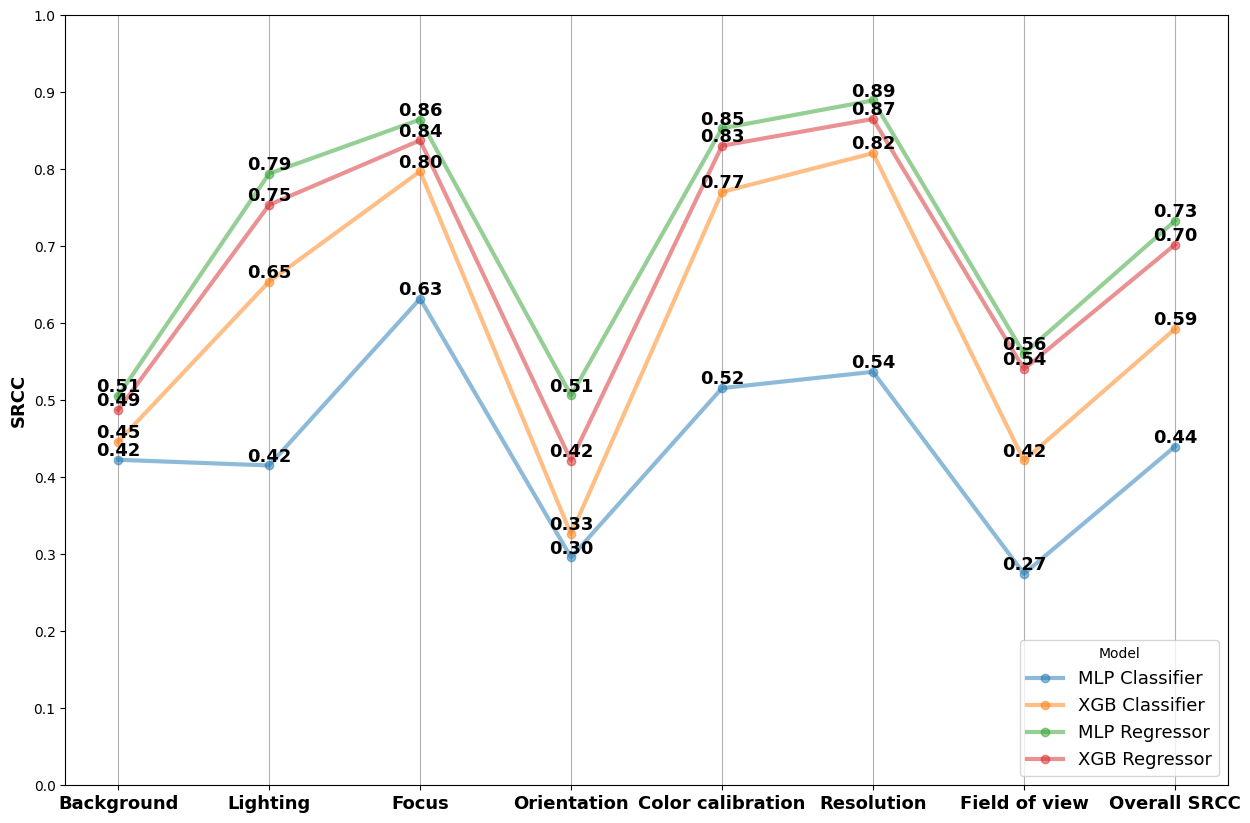
\includegraphics[keepaspectratio,width=15cm]{img/Model_SRCC.png}
    \caption{Parallel coordinate plot showing the best SRCC values for the four different models across the seven criteria and the overall SRCC. This plot highlights the performance of the MLP Regressor.}
    \label{fig:ModelSRCC}
\end{figure}

\subsection{Performance Metrics}
\label{subsec:PerformanceMetrics}
The performance of the final MLP regressor model on individual criteria is shown in \autoref{table:performance_metrics}. This table provides a comprehensive view of the model’s strengths and weaknesses, highlighting areas for improvement. The model was evaluated on 475 good quality Fitzpatrick images that were synthetically distorted using the distortion pipeline. \par
\begin{table}[h]
    \centering
    \begin{tabular}{|l|c|c|c|c|}
        \hline
        \textbf{Criteria} & \textbf{MAE} & \textbf{R\textsuperscript{2}} & \textbf{SRCC} & \textbf{Cohen's Kappa} \\
        \hline
        Background & 0.9684 & 0.2595 & 0.5422 & 0.4399 \\
        Lighting & 0.5726 & 0.6440 & 0.8028 & 0.7913 \\
        Focus & 0.4042 & 0.7385 & 0.8622 & 0.8568 \\
        Orientation & 0.9895 & 0.1824 & 0.4735 & 0.4102 \\
        Color calibration & 0.4905 & 0.7334 & 0.8622 & 0.8583 \\
        Resolution & 0.3642 & 0.7656 & 0.8722 & 0.8726 \\
        Field of view & 0.5474 & 0.5976 & 0.7710 & 0.7660 \\
        \hline
        \textbf{Overall} & \textbf{0.6195} & \textbf{0.5646} & \textbf{0.7507} & \textbf{0.7396} \\
        \hline
    \end{tabular}
    \caption{Performance Metrics for Each Distortion Criteria}
    \label{table:performance_metrics}
\end{table}

\clearpage
\subsection{Confusion Matrices}
\label{subsec:ConfusionMatrices}
In addition to numerical metrics, confusion matrices\footnote{from utils.visualization import plot\_all\_confusion\_matrices} were created for each criterion, as shown in \autoref{fig:confusion_matrices}. These matrices display where the model makes correct predictions and where it makes mistakes, showing a detailed view of its accuracy for each type of distortion. The comparison between actual and predicted scores helps identify specific areas where the model performs well and areas that need improvement. Furthermore, the confusion matrices also reveal any biases the model might have toward certain severity ranges, indicating whether it tends to predict only low or high severity levels, or if its predictions are skewed in some way. \par
\vspace{\baselineskip}
\begin{figure}[ht]
    \centering
    \begin{subfigure}[b]{0.32\textwidth}
        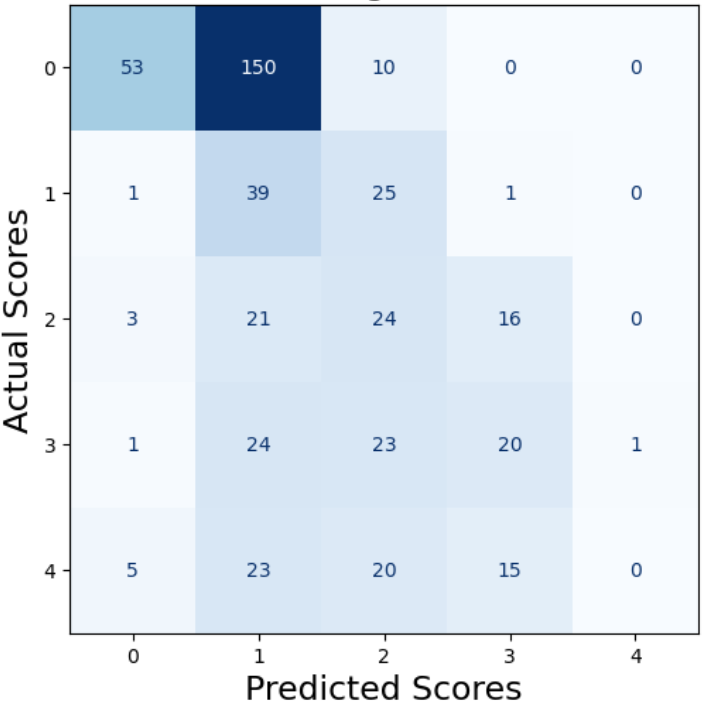
\includegraphics[width=\textwidth]{img/cm/bg.png}
        \caption{Background}
        \label{fig:cm_bg}
    \end{subfigure}
    \hfill
    \begin{subfigure}[b]{0.32\textwidth}
        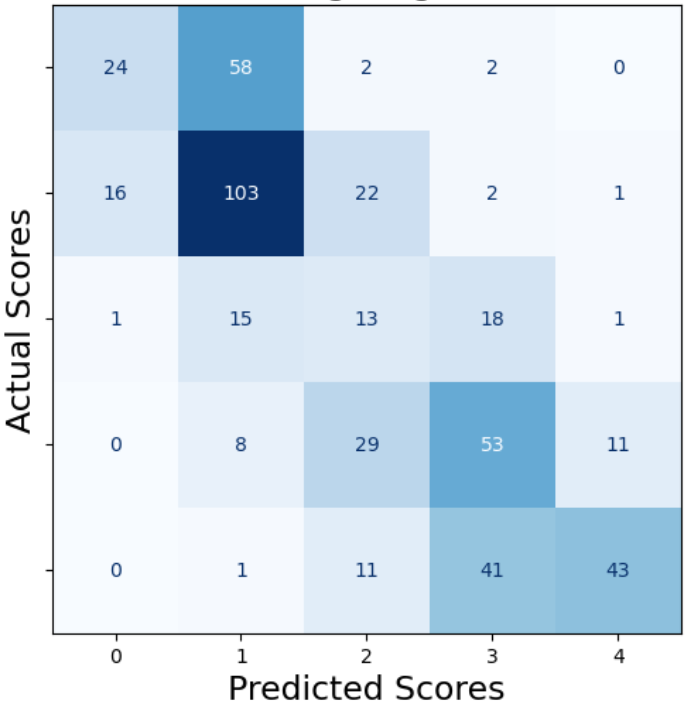
\includegraphics[width=\textwidth]{img/cm/light.png}
        \caption{Lighting}
        \label{fig:cm_light}
    \end{subfigure}
    \hfill
    \begin{subfigure}[b]{0.32\textwidth}
        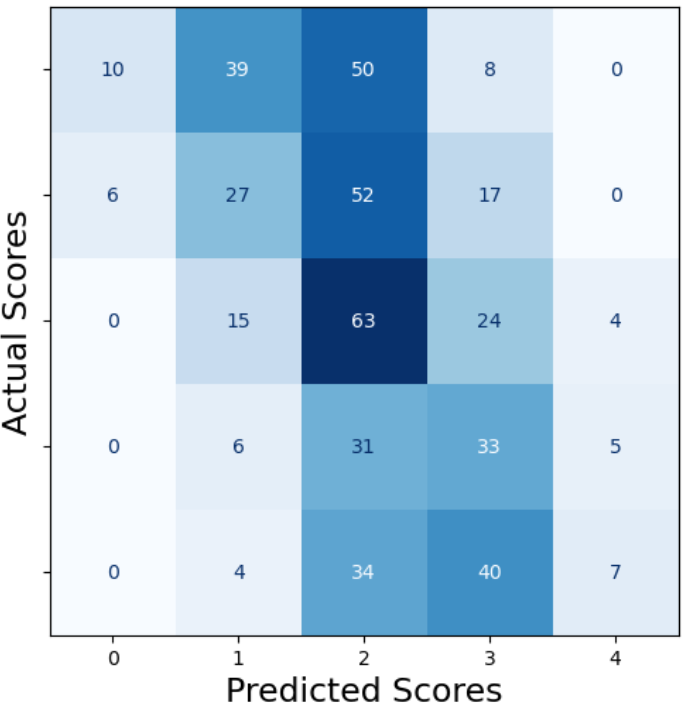
\includegraphics[width=\textwidth]{img/cm/orient.png}
        \caption{Orientation}
        \label{fig:cm_orient}
    \end{subfigure} 

    \begin{subfigure}[b]{0.24\textwidth}
        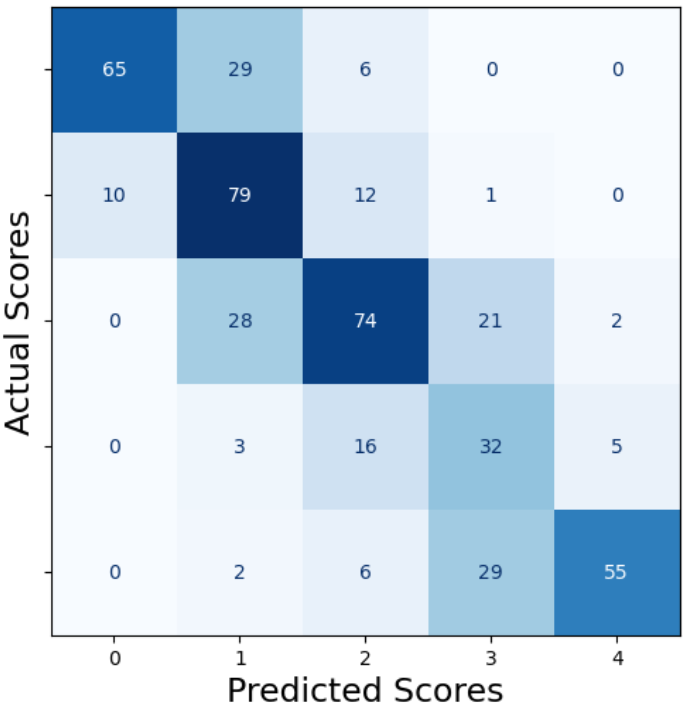
\includegraphics[width=\textwidth]{img/cm/foc.png}
        \caption{Focus}
        \label{fig:cm_foc}
    \end{subfigure}
    \hfill
    \begin{subfigure}[b]{0.24\textwidth}
        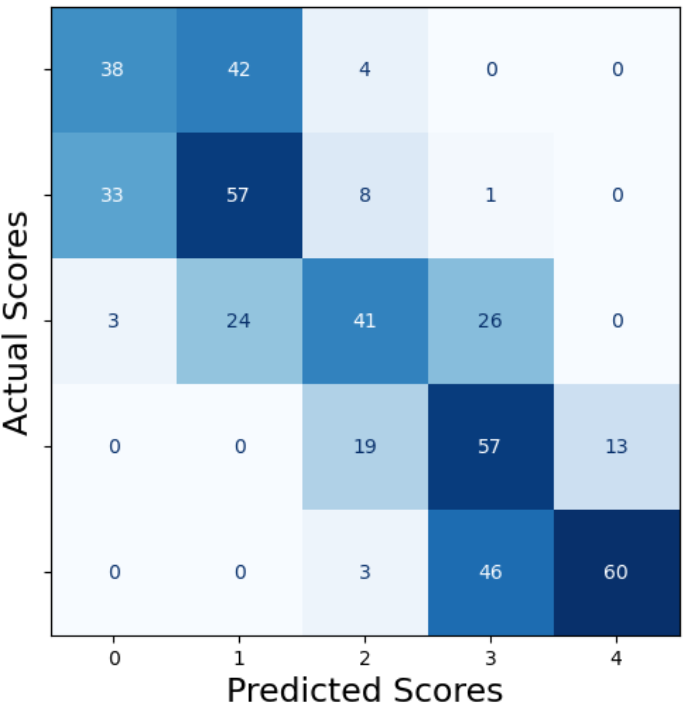
\includegraphics[width=\textwidth]{img/cm/cc.png}
        \caption{Color Calibration}
        \label{fig:cm_cc}
    \end{subfigure}
    \hfill
    \begin{subfigure}[b]{0.24\textwidth}
        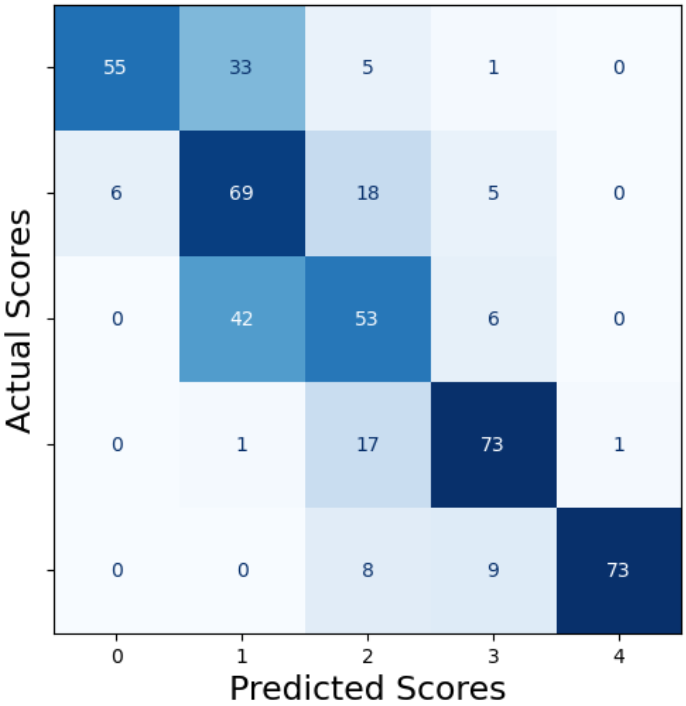
\includegraphics[width=\textwidth]{img/cm/res.png}
        \caption{Resolution}
        \label{fig:cm_res}
    \end{subfigure}
    \hfill
    \begin{subfigure}[b]{0.24\textwidth}
        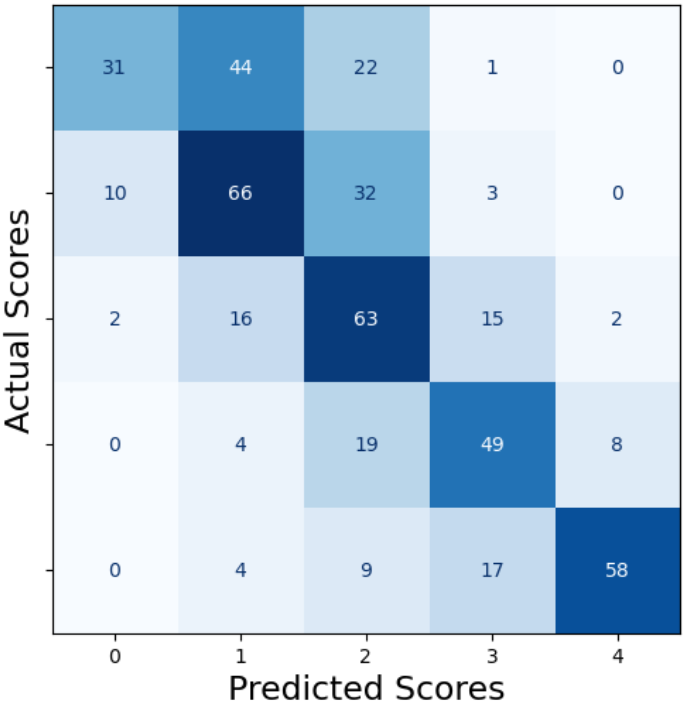
\includegraphics[width=\textwidth]{img/cm/fov.png}
        \caption{Field of View}
        \label{fig:cm_fov}
    \end{subfigure}
    \caption{Confusion matrices for the MLP Regressor model evaluated on the 475 images from the Fitzpatrick dataset. Each matrix corresponds to a specific distortion criterion and shows the actual scores on the y-axis and the predicted scores on the x-axis. Darker shades indicate higher counts, highlighting where the model's predictions match the actual values and where discrepancies occur.}
    \label{fig:confusion_matrices}
\end{figure}
\vspace{\baselineskip}
\noindent

\clearpage
\section{Model Predictions}
\label{sec:VisualizingPredictions}
To better understand the model’s performance on the two test sets (70 synthetic distorted images and 200 authentic images), radar charts\footnote{from utils.visualization import plot\_results} were created. These charts show the criteria on the outside, with severity ranges going from the center (0) to the outer edge (1), indicating high distortion for each criterion. These visualizations provide a clear and simple view of the model’s performance, showing its strengths and areas for improvement. They help identify specific cases where the model predicted the correct severity and where it struggled. The radar charts also make it easy to see which distortions the model handles well and which need more attention. \par
\subsection{Visualizations for Synthetic Distorted Images}
\label{subsec:SyntheticDistortedImages}
These visualizations, as shown in \autoref{fig:synthetic}, help to compare the model's predictions with the actual distortions introduced by the pipeline. This approach clearly demonstrates the model's ability to handle various types of distortions. \par
\vspace{\baselineskip}
\noindent
The first column shows the original image, the second displays the distorted image, the third contains the actual labels, and the fourth presents the model’s predictions. This setup makes it easy to compare the model’s predictions with the actual distortions. \par
\begin{figure}[ht]
    \centering
    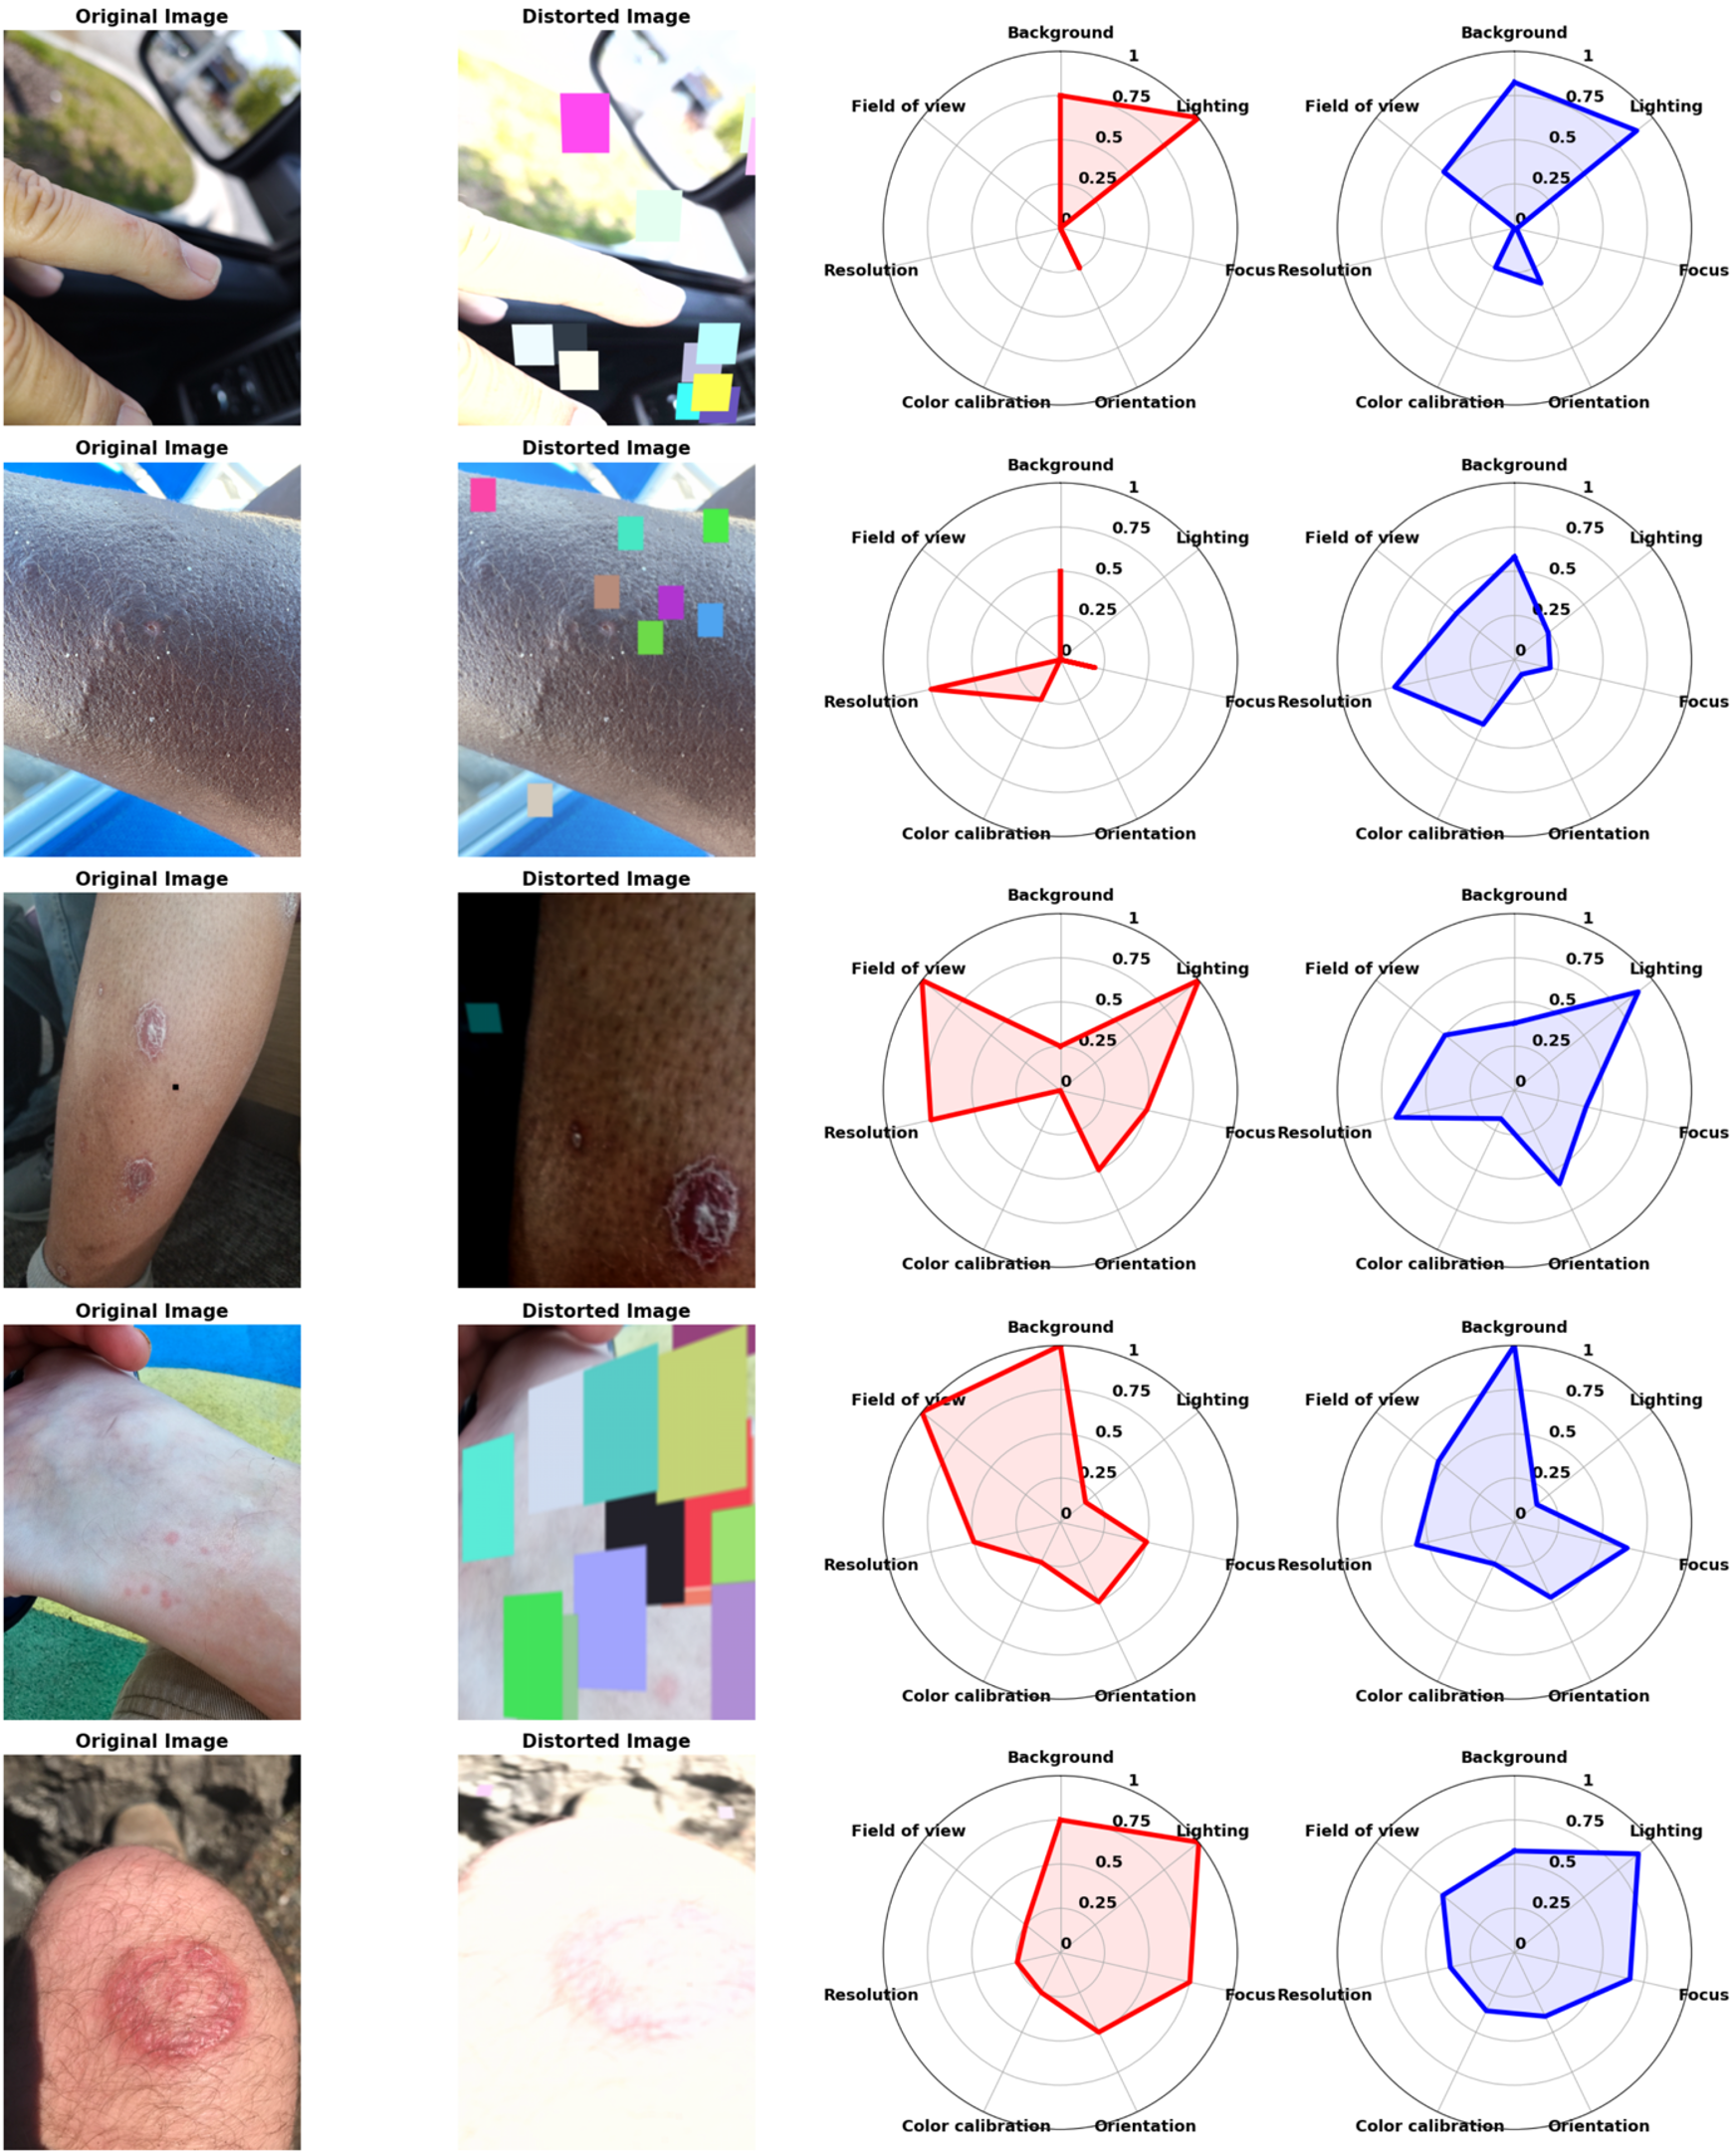
\includegraphics[keepaspectratio,width=15cm]{img/synthetic.png}
    \caption{Visualizations for the MLP Regressor model on 70 synthetic distorted images. The four-column layout shows the original image, the distorted image, the actual labels, and the model's predictions.}
    \label{fig:synthetic}
\end{figure}

\subsection{Visualizations for Authentic Images}
\label{subsec:AuthenticImages}
The visualizations, as shown in \autoref{fig:authentic}, compare the model's predictions with human-labeled scores. This method highlights the model's performance in real-world scenarios, showing its strengths and areas for improvement. \par
\vspace{\baselineskip}
\noindent
The first column shows the image, the second column displays the human-labeled scores, and the third column presents the model’s predictions. This comparison helps show how well the model’s predictions align with the human evaluations. \par
\begin{figure}[ht]
    \centering
    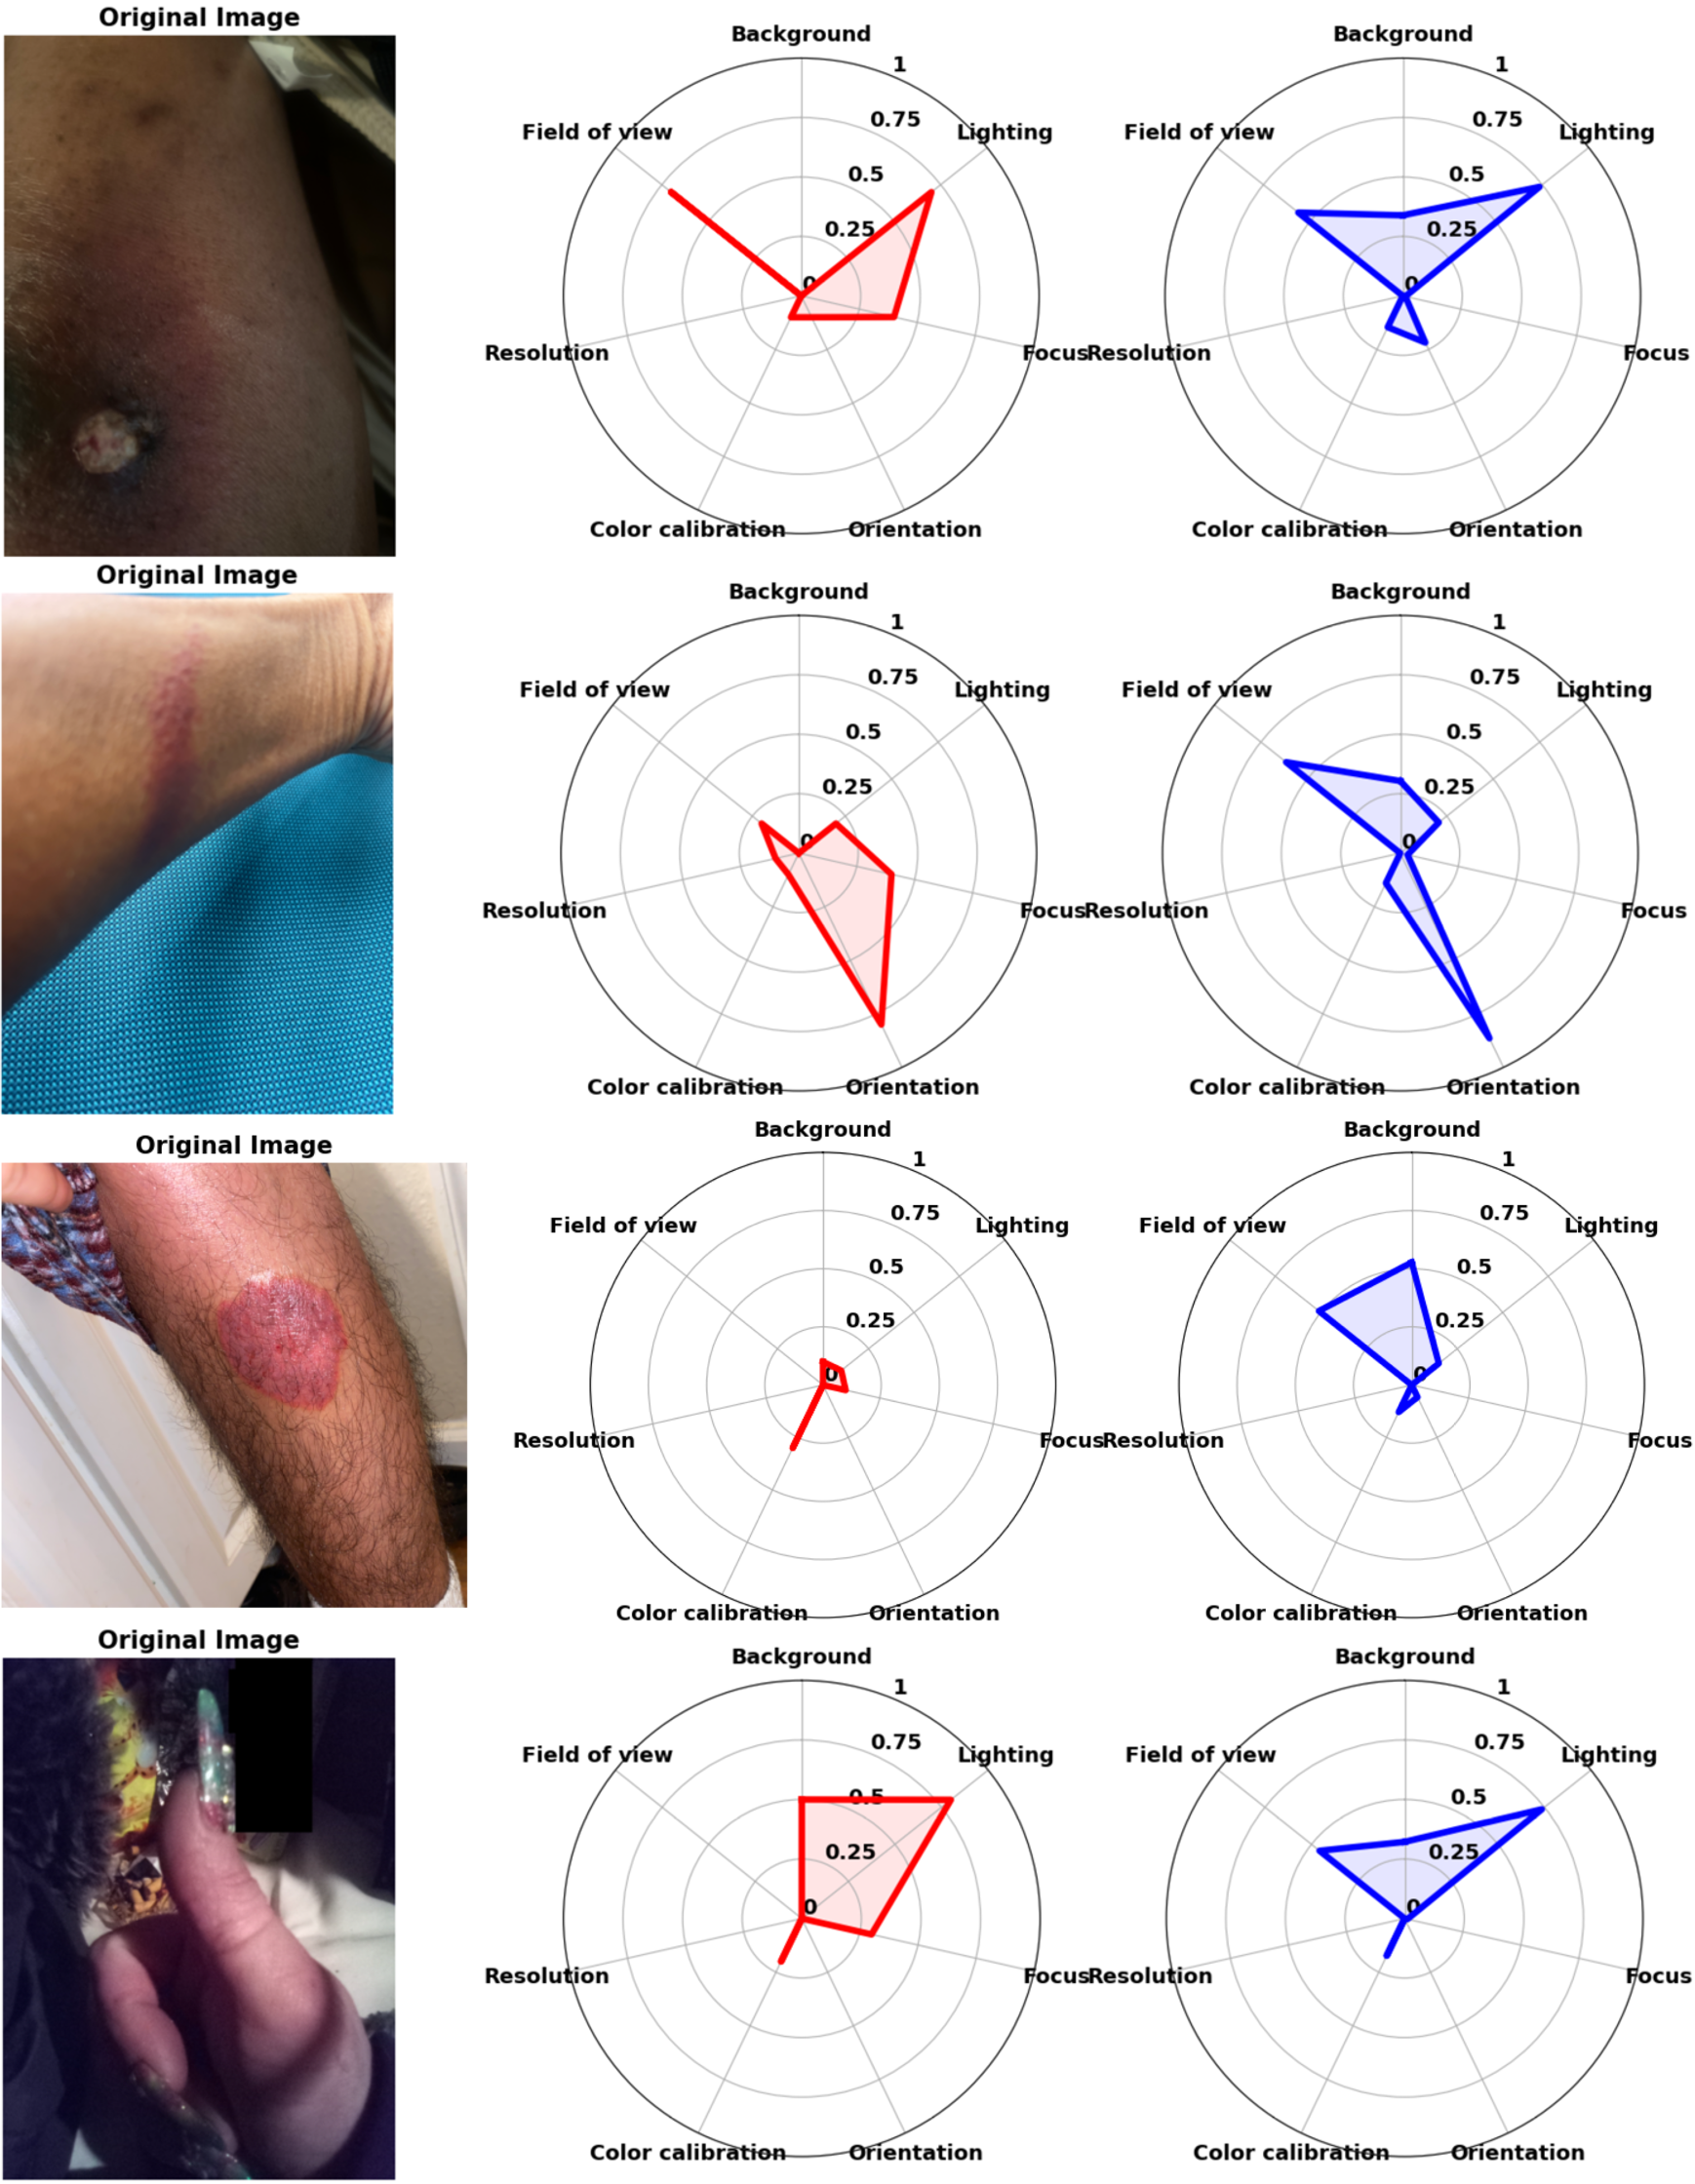
\includegraphics[keepaspectratio,width=15cm]{img/authentic.png}
    \caption{Visualizations for the MLP Regressor model on 200 authentic images. The three-column layout shows the image, the human-labeled scores, and the model's predictions.}
    \label{fig:authentic}
\end{figure}
\clearpage
\section{Assessing Training and Testing Images Quality}
\label{sec:TestingFilteredImages}
To verify the quality of the images used for training and see how they change after synthetic distortion, radar charts were created. These charts show the quality of the original training images and how they are affected by the distortions. Additionally, the quality of both the synthetic and authentic test images is assessed using the same method. These radar charts show a simple visual representation of the quality and the level of distortion across the seven criteria. \par
\subsection{Training Images Quality}
\label{subsec:TrainingImagesQuality}
\subsubsection{SCIN Dataset}
\label{subsubsec:SCINDataset}
\begin{figure}[ht]
    \centering
    \begin{subfigure}[b]{0.48\textwidth}
        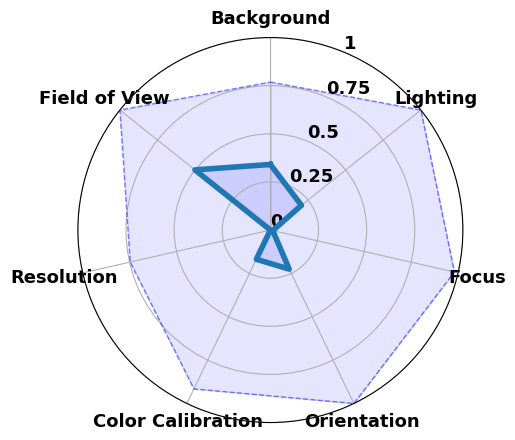
\includegraphics[width=\textwidth]{img/hept/SCIN10k.png}
        \caption{SCIN Images}
        \label{fig:SCIN10k}
    \end{subfigure}
    \hfill
    \begin{subfigure}[b]{0.48\textwidth}
        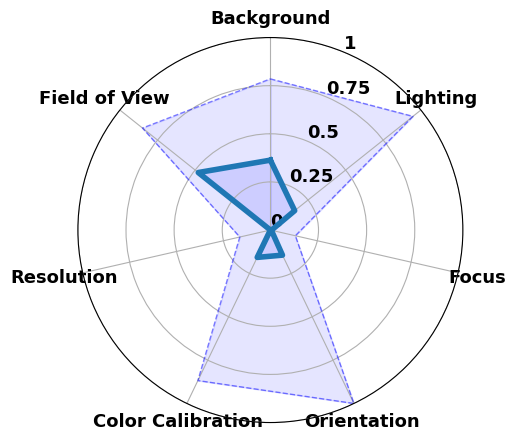
\includegraphics[width=\textwidth]{img/hept/SCIN.png}
        \caption{Filtered SCIN Images}
        \label{fig:SCIN}
    \end{subfigure}
    \hfill
    \caption{Radar charts for the SCIN dataset. (a) Original images from the SCIN dataset (10'379 images). (b) Filtered good quality images (475 images).}
    \label{fig:SF}
\end{figure}
\clearpage
\subsubsection{Fitzpatrick Dataset}
\label{subsubsec:FitzpatrickDataset}
\begin{figure}[ht]
    \centering
    \begin{subfigure}[b]{0.48\textwidth}
        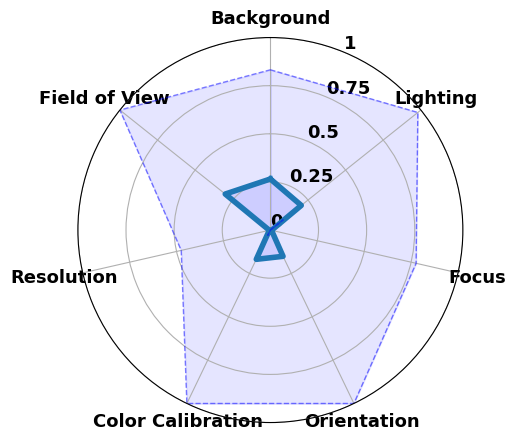
\includegraphics[width=\textwidth]{img/hept/Fitzpatrick17k.png}
        \caption{Fitzpatrick Images}
        \label{fig:Fitzpatrick17K}
    \end{subfigure}
    \hfill
    \begin{subfigure}[b]{0.48\textwidth}
        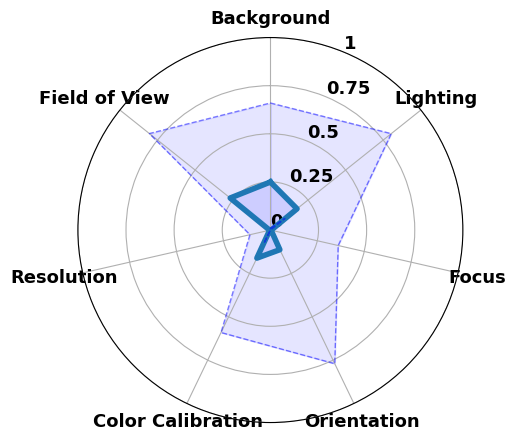
\includegraphics[width=\textwidth]{img/hept/F17K.png}
        \caption{Filtered Fitzpatrick Images}
        \label{fig:F17K}
    \end{subfigure}
    \hfill
    \caption{Radar charts for the Fitzpatrick dataset. (a) Original images from the Fitzpatrick dataset (16'577 images). (b) Filtered good quality images (475 images).}
    \label{fig:FF}
\end{figure}

\subsubsection{Combined Dataset}
\label{subsubsec:CombinedDataset}
\begin{figure}[ht]
    \centering
    \begin{subfigure}[b]{0.48\textwidth}
        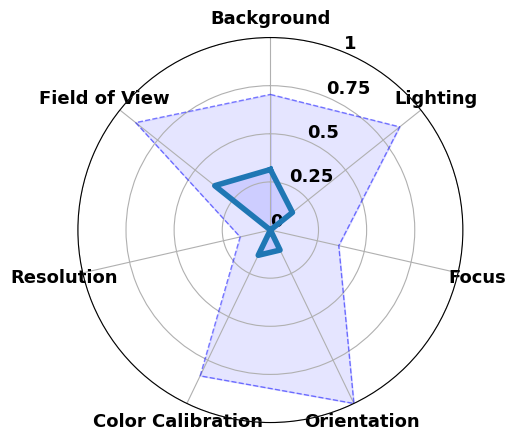
\includegraphics[width=\textwidth]{img/hept/combined.png}
        \caption{Combined SCIN and Fitzpatrick Images}
        \label{fig:combined}
    \end{subfigure}
    \hfill
    \begin{subfigure}[b]{0.48\textwidth}
        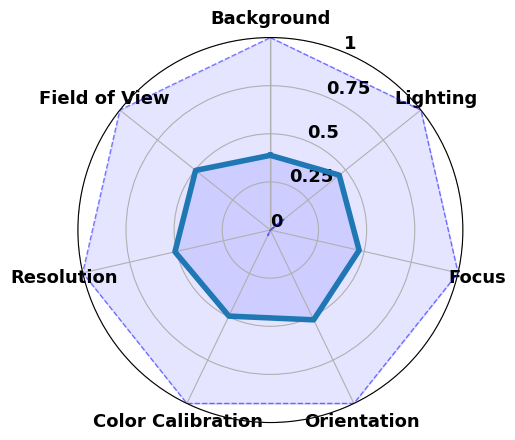
\includegraphics[width=\textwidth]{img/hept/comb_synthetic.png}
        \caption{Synthetically Distorted Images}
        \label{fig:comb_synthetic}
    \end{subfigure}
    \hfill
    \caption{Combined dataset analysis. (a) Combined SCIN and Fitzpatrick images (950 images). (b) Synthetically distorted images.}
    \label{fig:CF}
\end{figure}
\clearpage
\subsection{Test Images Quality}
\label{subsec:TestImagesQuality}
\subsubsection{Synthetic Test Images}
\label{subsubsec:SyntheticTestImages}
\begin{figure}[ht]
    \centering
    \begin{subfigure}[b]{0.48\textwidth}
        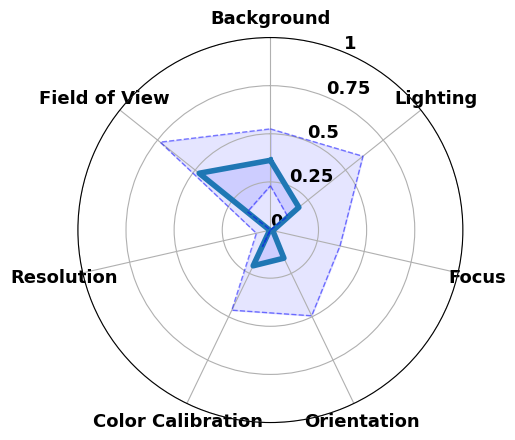
\includegraphics[width=\textwidth]{img/hept/test_70.png}
        \caption{Filtered Test Images}
        \label{fig:test_70}
    \end{subfigure}
    \hfill
    \begin{subfigure}[b]{0.48\textwidth}
        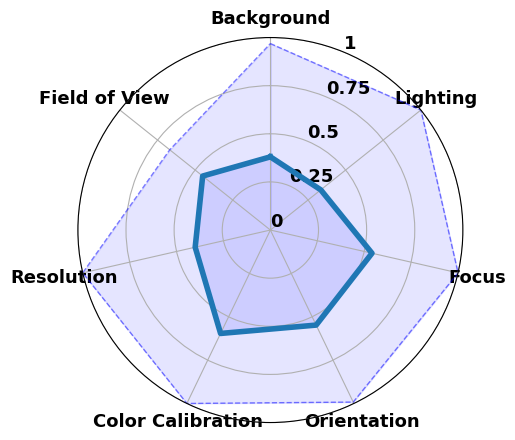
\includegraphics[width=\textwidth]{img/hept/test_70_synthetic.png}
        \caption{Synthetically Distorted Test Images}
        \label{fig:test_70_synthetic}
    \end{subfigure}
    \hfill
    \caption{Synthetic test set analysis. (a) Filtered good quality test images (70 images, independent of training set). (b) Synthetically distorted test images.}
    \label{fig:T1}
\end{figure}

\subsubsection{Authentic Test Images}
\label{subsubsec:AuthenticTestImages}
\begin{figure}[ht]
    \centering
    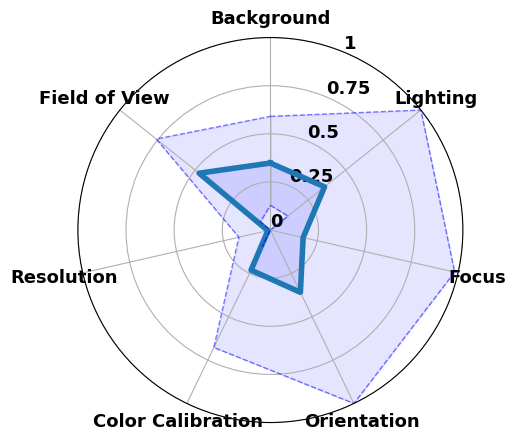
\includegraphics[keepaspectratio,width=7cm]{img/hept/test_200.png}
    \caption{Authentic test set from the SCIN dataset, independent of the training images, showing real-world distortions.}
    \label{fig:T2}
\end{figure}